% Copyright (c) 2023-2025
% This file is part of sep3cs.
%
% sep3cs is free software: you can redistribute it and/or modify
% it under the terms of the GNU General Public License as published by
% the Free Software Foundation, either version 3 of the License, or
% (at your option) any later version.
%
% sep3cs is distributed in the hope that it will be useful,
% but WITHOUT ANY WARRANTY; without even the implied warranty of
% MERCHANTABILITY or FITNESS FOR A PARTICULAR PURPOSE.  See the
% GNU General Public License for more details.
%
% You should have received a copy of the GNU General Public License
% along with sep3cs. If not, see <http://www.gnu.org/licenses/>.
%
\section{Funcionalidades}

\begin{figure}[H]
  \centering
  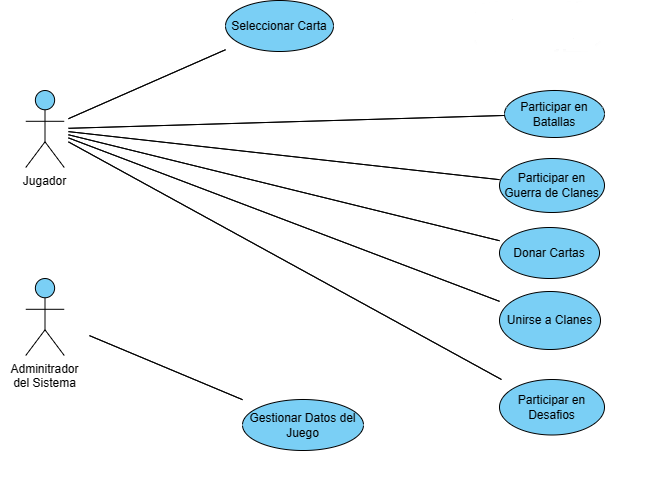
\includegraphics[width=0.5\textwidth]{../images/comic_use_cases.png}
\end{figure}

\begin{enumerate}
  \item Seleccionar Carta: Los jugadores pueden seleccionar cartas para usar en las batallas. Cada carta tiene habilidades y estadísticas únicas que pueden influir en el resultado de una batalla.
  \item Donar Carta: Los jugadores pueden donar cartas a otros miembros de su clan. Esto puede ayudar a los miembros del clan a mejorar sus mazos y avanzar en el juego.
  \item Unirse a Clanes: Los jugadores pueden unirse a clanes existentes o crear nuevos clanes. Dentro de un clan, los jugadores pueden colaborar, compartir cartas y participar en guerras de clanes juntos.
  \item Participar en Batallas: Los jugadores pueden participar en batallas uno a uno para ganar trofeos. El objetivo es destruir las torres del oponente mientras defienden las suyas.
  \item Participar en Desafíos: Los desafíos son eventos especiales donde los jugadores pueden ganar recompensas adicionales. Los jugadores deben acumular victorias en estos eventos para obtener las recompensas.
  \item Participar en Guerras de Clanes: Las guerras de clanes son eventos competitivos donde varios clanes compiten entre sí por trofeos y recompensas.
  \item Gestionar Datos del Juego: El administrador del sistema recopila y analiza datos sobre el comportamiento del juego para ayudar a diseñar nuevas formas de juego que atraigan a nuevos jugadores y mantengan a los actuales jugando.
\end{enumerate}

\begin{figure}[H]
  \centering
  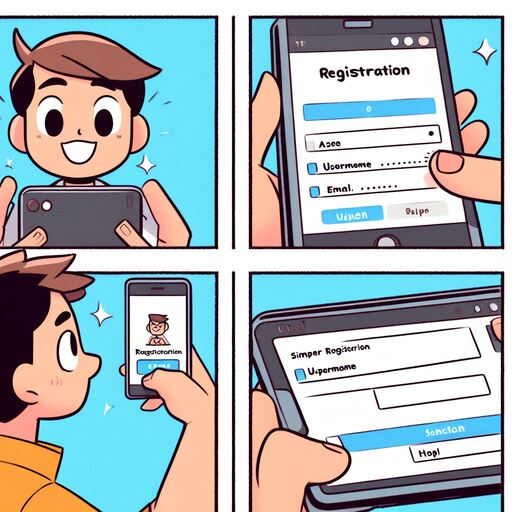
\includegraphics[width=0.8\textwidth]{../images/comic_registration.jpeg}
  \caption{Muestra a un  usuario registrándose en tu aplicación}
\end{figure}

\begin{figure}[H]
  \centering
  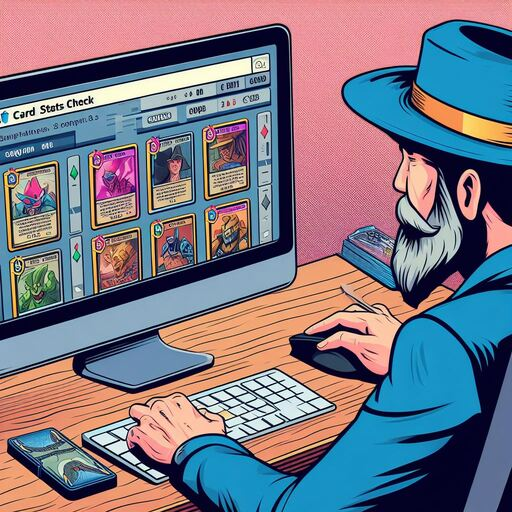
\includegraphics[width=0.8\textwidth]{../images/comic_query_card_stats.jpeg}
  \caption{Muestra al usuario consultando las estadísticas de diferentes cartas}
\end{figure}

\begin{figure}[H]
  \centering
  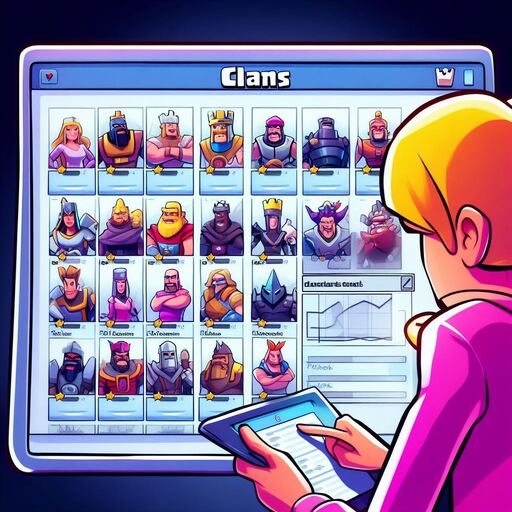
\includegraphics[width=0.8\textwidth]{../images/comic_query_clan_stats.jpeg}
  \caption{Muestra al usuario consultando las estadísticas de diferentes clanes}
\end{figure}

\begin{figure}[H]
  \centering
  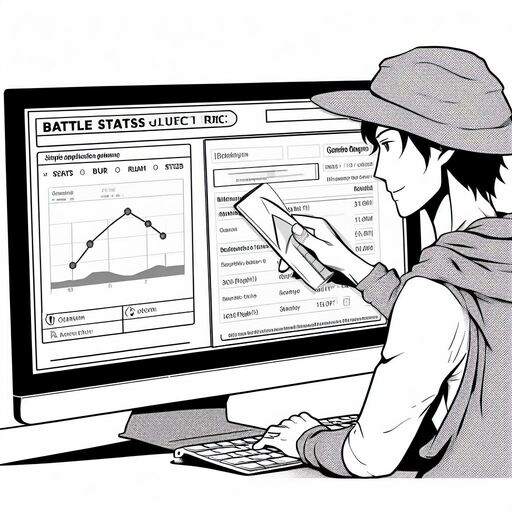
\includegraphics[width=0.8\textwidth]{../images/comic_query_match_stats.jpeg}
  \caption{Muestra al usuario consultando las estadísticas de diferentes batallas}
\end{figure}

\begin{figure}[H]
  \centering
  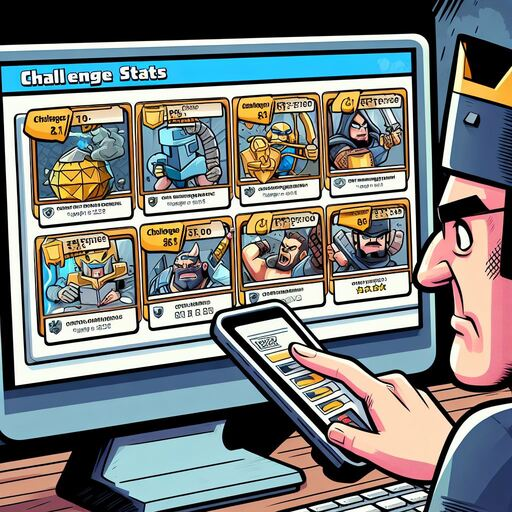
\includegraphics[width=0.8\textwidth]{../images/comic_query_challenge_stats.jpeg}
  \caption{Muestra al usuario consultando las estadísticas de diferentes desafíos}
\end{figure}

\begin{figure}[H]
  \centering
  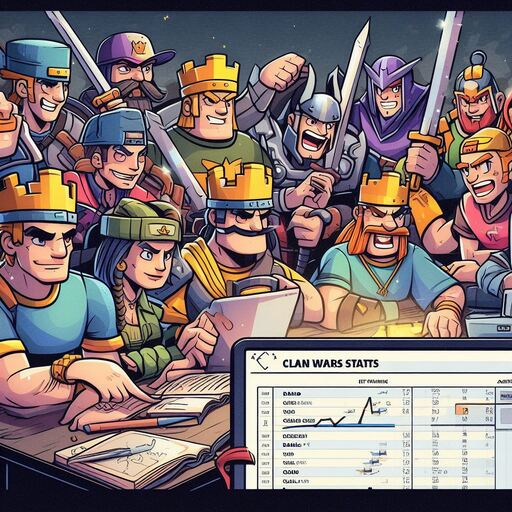
\includegraphics[width=0.8\textwidth]{../images/comic_query_clan_war_stats.jpeg}
  \caption{Muestra al usuario consultando las estadísticas de diferentes guerras de clanes}
\end{figure}

\begin{figure}[H]
  \centering
  
\includegraphics[width=0.8\textwidth]{../images/comic_administrator.jpeg}
  \caption{Muestra al administrador del sistema utilizando una interfaz administrativa para ver estadísticas del uso de la aplicación, ajustar la configuración y añadir nuevas características.}
\end{figure}
